% !TeX program = xelatex
\documentclass[final,5p,times,twocolumn,nonatbib]{elsarticle}

\newif\ifBSPCtwocolumn
\BSPCtwocolumntrue
\usepackage{xeCJK}
% Fandol is distributed with TeX Live and is available on Overleaf.
\setCJKmainfont[
  BoldFont=FandolHei-Regular.otf,
  ItalicFont=FandolKai-Regular.otf,
  BoldItalicFont=FandolHei-Regular.otf
]{FandolSong-Regular.otf}
\setCJKsansfont{FandolHei-Regular.otf}
\setCJKmonofont{FandolFang-Regular.otf}
\renewcommand{\figurename}{图}
\renewcommand{\tablename}{表}
% Shared packages and formatting-only compatibility definitions.
\usepackage{amsmath,amssymb}
\usepackage{array,booktabs,tabularx}
\usepackage{caption}
\DeclareCaptionFont{bspctablefont}{\fontsize{8}{10}\selectfont}
\captionsetup[table]{font=bspctablefont,labelfont=normalfont,position=top,skip=4pt}
\captionsetup[figure]{position=bottom}
\newcommand{\BSPCtableformat}{\fontsize{8}{10}\selectfont\setlength{\tabcolsep}{2pt}\renewcommand{\arraystretch}{1.12}}
\usepackage{placeins}
\usepackage{flafter}
\usepackage{dblfloatfix}
\usepackage{cite}

% Preserve the approved source behavior: two consecutive references form a range.
\makeatletter
\def\@compress@cite#1#2#3{%
  \ifnum\@cite@incr=\z@
    \advance\@tempcnta\@cclvi
    \ifnum #1=\@tempcnta
      \def\@h@ld{\citedash\@cite@out{#3}}%
      \mathchardef\@cite@incr=\@cclvi
    \else
      \advance\@tempcnta-\@cclv
      \ifnum #1=\@tempcnta
        \def\@h@ld{\citedash\@cite@out{#3}}%
        \mathchardef\@cite@incr=\@ne
      \else
        \@citea\@cite@out{#3}%
      \fi
    \fi
  \else
    \advance\@tempcnta\@cite@incr
    \ifnum #1=\@tempcnta
      \def\@h@ld{\citedash\@cite@out{#3}}%
    \else
      \@h@ld\@citea\@cite@out{#3}%
      \let\@h@ld\@empty
      \mathchardef\@cite@incr=\z@
    \fi
  \fi
  \@tempcnta#1\let\@citea\citepunct
}
\makeatother
\renewcommand{\citedash}{\hbox{--}\penalty\citepunctpenalty}

\usepackage{url}
\usepackage[hidelinks]{hyperref}

\graphicspath{{figures/}}
\newcolumntype{Y}{>{\raggedright\arraybackslash}X}
\newcolumntype{Z}{>{\centering\arraybackslash}X}
\setlength{\emergencystretch}{1em}
\hyphenation{echo-car-di-og-ra-phy}

% The same body file expands to ordinary floats in preprint mode and to
% full-width floats for wide items in the 5p two-column preview. Define the
% selected environment statically so a conditional never crosses a float group.
\ifBSPCtwocolumn
  \newenvironment{bspcwidefigure}[1][!t]{\begin{figure*}[#1]}{\end{figure*}}
  \newenvironment{bspclabelefficiencyfigure}{\begin{figure*}[t]}{\end{figure*}}
  \newenvironment{bspcwidetable}[1][!t]{\begin{table*}[#1]}{\end{table*}}
  \newcommand{\BSPCcompacttableformat}{\BSPCtableformat}
  \newcommand{\BSPCstrictnopretraining}{\shortstack[l]{Strict no-\\pretraining}}
  \newcommand{\BSPCstorelabelefficiencyinterpretation}[1]{\gdef\BSPClabelefficiencyinterpretation{#1}}
  \newcommand{\BSPCemitlabelefficiencyinterpretation}{\BSPClabelefficiencyinterpretation}
  % Keep prose available to backfill pages while wide floats wait for their
  % next legal top position. Source order and the double-float limit retain the
  % architecture sequence without forcing a sparse transition page.
  \newcommand{\BSPCseparatearchitecturefigures}{}
  \newcommand{\BSPCseparatelabelefficiencyfloats}{}
  \newcommand{\BSPCseparateresultfloatgroups}{}
  \newcommand{\BSPCkeependpointorder}{}
\else
  % Preprint mode can use here/top/bottom/float-page placement.  The body keeps
  % the same scientific float declarations as the two-column build.
  \newenvironment{bspcwidefigure}[1][!htbp]{\begin{figure}[!htbp]}{\end{figure}}
  \newenvironment{bspclabelefficiencyfigure}{\begin{figure}[!htbp]}{\end{figure}}
  \newenvironment{bspcwidetable}[1][!htbp]{\begin{table}[!htbp]}{\end{table}}
  \newcommand{\BSPCcompacttableformat}{\BSPCtableformat}
  \newcommand{\BSPCstrictnopretraining}{Strict no-pretraining}
  \newcommand{\BSPCstorelabelefficiencyinterpretation}[1]{#1}
  \newcommand{\BSPCemitlabelefficiencyinterpretation}{}
  \newcommand{\BSPCseparatearchitecturefigures}{}
  \newcommand{\BSPCseparatelabelefficiencyfloats}{}
  \newcommand{\BSPCseparateresultfloatgroups}{}
  \newcommand{\BSPCkeependpointorder}{}
\fi

% Keep compact tables next to their discussion at a fixed font size.
\setcounter{topnumber}{1}
\setcounter{bottomnumber}{1}
\setcounter{totalnumber}{2}
\renewcommand{\topfraction}{0.72}
\renewcommand{\bottomfraction}{0.55}
\renewcommand{\textfraction}{0.22}
\renewcommand{\floatpagefraction}{0.78}
\ifBSPCtwocolumn
  \setcounter{dbltopnumber}{2}
  \renewcommand{\dbltopfraction}{0.80}
  \renewcommand{\dblfloatpagefraction}{0.78}
\fi
\setlength{\textfloatsep}{12pt plus 2pt minus 2pt}
\setlength{\floatsep}{10pt plus 2pt minus 2pt}
\setlength{\intextsep}{10pt plus 2pt minus 2pt}

% Numeric Elsevier-derived bibliography with user-requested author shortening.
% Keep reference entries compact without changing their type size.
\let\BSPCoriginalthebibliography\thebibliography
\renewcommand{\thebibliography}[1]{%
  \BSPCoriginalthebibliography{#1}%
  \setlength{\itemsep}{2pt plus 0.5pt minus 0.5pt}%
  \setlength{\parsep}{0pt}%
}
\newcommand{\BSPCprintbibliography}{%
  \begingroup
  \footnotesize
  \bibliographystyle{bspc-num-five}%
  \bibliography{references_bspc_with_figs_v1}%
  \endgroup
}

\setcounter{secnumdepth}{3}

\journal{Biomedical Signal Processing and Control}

\begin{document}
\begin{frontmatter}

\title{基于全卷积掩码预训练与一维 ConvNeXt 的心电结构性心脏病筛查}

\begin{abstract}
超声心动图用于确认结构性心脏病（structural heart disease，SHD），十二导联心电图（ECG）则提供了广泛可得的结构异常预测信号。从未标注 ECG 学习表征可降低模型对配对心电图--超声心动图训练标签的依赖。本研究构建 ECG-FCMAE，将同步导联间共享的时间片段掩码、一维 ConvNeXt 编码器及Tabular inputs 条件调制结合，在 EchoNext 回顾性队列中比较具有相同下游架构和训练协议的预训练模型与随机初始化对照。三个下游种子中，预训练模型的 Overall SHD 受试者工作特征曲线下面积（AUROC）为 $0.8521\pm0.0008$，随机初始化对照为 $0.8448\pm0.0001$。三种子概率集成的 AUROC 差值为 $+0.0061$（患者级配对 95\% 置信区间：$[0.0034,\,0.0088]$）。在使用 1\%、5\%、10\%、30\% 和 100\% 有标签训练记录时，预训练均提高 AUROC 和精确率--召回率曲线下面积，所有配对区间均排除 0。AUROC 收益在 1\% 时最大，为 $+0.0323$（95\% 置信区间：$[0.0239,\,0.0408]$）。结果表明，掩码 ECG 预训练提高了 SHD 判别性能和标签利用效率。
\end{abstract}

\begin{keyword}
结构性心脏病 \sep 十二导联心电图 \sep 掩码自监督学习 \sep 表征学习 \sep 标签利用效率
\end{keyword}

\end{frontmatter}
\raggedbottom

\section{引言}
\label{sec:introduction}

结构性心脏病包括心室功能、心肌结构和瓣膜功能等异常，其确认和分型通常依赖超声心动图等成像检查\cite{lang2015chamber,otto2021valvular}。十二导联心电图检查便捷、成本较低且广泛存在于临床流程中。人工智能心电图研究表明，波形能够编码与潜在结构异常相关、且难以由人工稳定识别的预测信息\cite{siontis2021aiecg}。因此，从心电图检测超声心动图定义的 SHD，为研究基于心电图评分的进一步检查优先排序提供了基础。

既往深度学习研究已从心电图波形或图像识别左心室收缩功能障碍、瓣膜病及更广泛的超声心动图异常\cite{attia2019contractile,elias2022valvenet,ulloacerna2022rechommend,poterucha2025echonext,dhingra_present_shd_2025,aminorroaya_adapt_shd_2025}。这些工作在不同队列、输入形式和预测目标中建立了电活动与结构表型的关联\cite{avula2023ecgreview}。对配对 ECG--超声心动图标签的依赖，推动了从未标注波形学习可复用表征的研究。

监督式人工智能心电图模型依赖定义一致的 ECG--超声心动图配对标签。EchoNext 将 ECG 记录与超声心动图来源的二分类异常标签相配对\cite{elias2026echonextdata}；相较于日常积累的未标注心电波形，可用于特定异常目标训练的配对记录受到标签构建过程的限制。已有掩码预训练研究将有限标注条件作为独立评价维度\cite{sawano_masked_lvsd_2024,ran_joint_masking_2024}。核心问题是未标注波形能否提供可迁移的初始化，以及这一初始化能否降低下游任务对配对标签的需求。

心电图自监督学习已探索跨视图对比学习和导联关系建模\cite{kiyasseh2021clocs,mehari2022ssl,oh2022leadagnostic}，也采用时间--导联变换判别与掩码重建学习标签无关的表示\cite{zhang_reverse_2023,zhang2023maefe,na2024stmem,ran_joint_masking_2024}。掩码预训练已在左心室收缩功能障碍和有限标注场景中得到评价\cite{sawano_masked_lvsd_2024}，而更广泛的基础模型基准表明，下游收益会随架构和任务而变化\cite{almasud2026benchmark}。因此，在同步十二导联 ECG 的多目标二分类 SHD 任务中，卷积式掩码预训练能否相对同架构随机初始化产生可重复收益，仍需直接检验。

本研究将全卷积掩码自编码适配于同步十二导联 ECG，构建 ECG-FCMAE。跨导联共享的时间片段掩码保留重建过程中的时间对齐；迁移后的编码器结合一维 ConvNeXt、高效通道注意力、多尺度时间汇聚与七个表格变量的条件调制\cite{liu2022convnext,woo2023convnextv2,wang2020ecanet,perez2018film}。预训练及下游架构见图~\ref{fig:architecture}。

在架构、输入、数据划分、优化和模型选择规则相同的条件下，本研究比较预训练与随机初始化，以隔离初始化策略的影响。随后在五个有标签训练记录比例下评价标签效率，并分析表格信息、不同预测目标及导联配置对应的性能变化。

\section{材料与方法}
\label{sec:methods}

\subsection{研究数据集与队列}
\label{sec:cohort}

本研究使用 EchoNext 心电图--超声心动图配对队列\cite{elias2026echonextdata}。预定义训练集、验证集和测试集分别包含 $72{,}475$、$4{,}626$ 和 $5{,}442$ 条心电图记录，对应 $26{,}218$、$4{,}626$ 和 $5{,}442$ 名患者（表~\ref{tab:cohort}）。三个数据集的患者集合互不重叠；训练集允许同一患者贡献多条记录，验证集和测试集每位患者各保留一条记录。另有 $17{,}457$ 条未进入预定义划分的记录不纳入分析。模型开发和选择仅使用训练集与验证集，测试集在模型选择完成后用于最终评价。

\begin{table}[!htbp]
\centering
\BSPCtableformat

\caption{预定义队列划分。训练集允许重复患者记录；验证集和测试集每位患者一条记录。}
\label{tab:cohort}
\begin{tabular}{lrr}
\toprule
数据集 & 心电图记录数 & 患者数 \\
\midrule
训练集 & 72,475 & 26,218 \\
验证集 & 4,626 & 4,626 \\
测试集 & 5,442 & 5,442 \\
\bottomrule
\end{tabular}

\end{table}

整体研究路径与评价框架见图~\ref{fig:study_framework}。该图概括患者级数据划分、掩码预训练向下游任务的初始化迁移、12 个预测目标，以及主要与支持性评价设计；具体真实标签定义和模型细节在后续小节给出。

\begin{bspcwidefigure}[!t]
\centering
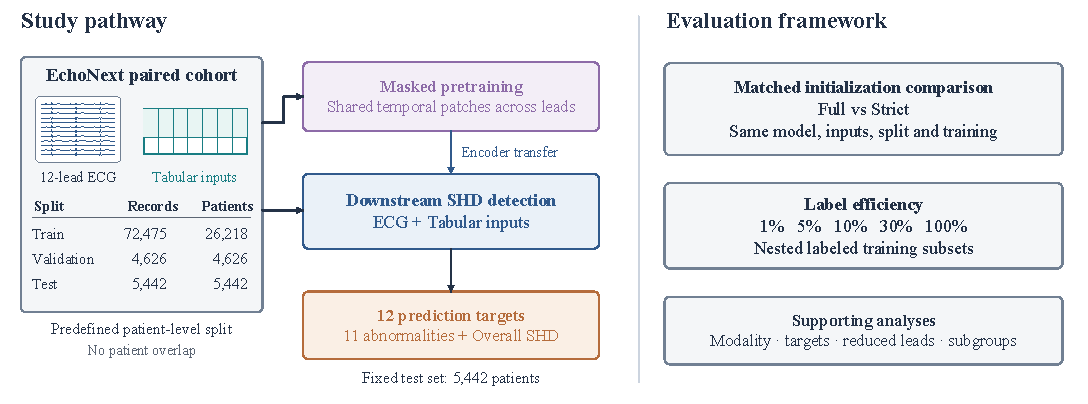
\includegraphics[width=\textwidth]{fig1_study_pathway_revised.pdf}
\caption{研究路径与评价框架。EchoNext 回顾性 ECG--超声心动图配对队列按患者划分为训练集、验证集和测试集。训练集十二导联 ECG 采用跨导联共享时间片段掩码进行自监督预训练，并将预训练初始化迁移至结合 7 个表格变量的下游 SHD 模型；超声心动图仅用于定义真实标签。模型产生 12 个目标特异输出，包括 11 种具体异常和 Overall SHD。评价框架包括预训练初始化与随机初始化的匹配比较，使用 1\%、5\%、10\%、30\% 和 100\% 有标签训练数据的标签效率分析，以及模态/表格信息、各预测目标和少导联分析。}
\label{fig:study_framework}
\end{bspcwidefigure}

\subsection{预测目标与真实标签定义}
\label{sec:outcomes}

模型同时预测 11 种由超声心动图定义的具体异常和 Overall SHD\cite{elias2026echonextdata}。11 种具体异常的判定标准依次为：左心室射血分数（LVEF）$\leq45\%$；左心室壁厚增加，即室间隔或左心室后壁舒张期厚度的较大值 $\geq13$~mm；中度及以上主动脉瓣狭窄；中度及以上主动脉瓣反流；中度及以上二尖瓣反流；中度及以上三尖瓣反流；中度及以上肺动脉瓣反流；中度及以上右心室收缩功能障碍；中量或大量心包积液；肺动脉收缩压（PASP）$\geq45$~mmHg；以及三尖瓣反流最大速度（TR Vmax）$\geq3.2$~m/s。记 $y_k\in\{0,1\}$ 为第 $k$ 种具体异常的真实标签，$y_{\mathrm{SHD}}\in\{0,1\}$ 为 Overall SHD 的真实标签。Overall SHD 的真实标签定义为
\begin{equation}
y_{\mathrm{SHD}}=\max\{y_1,y_2,\ldots,y_{11}\}.
\label{eq:overall_shd}
\end{equation}
当至少一种具体异常标签为阳性时，Overall SHD 标签为 1；当全部 11 种标签为阴性时，其标签为 0。最终分类层输出一个 12 维 logit 向量，每个元素对应一个预测目标。逐元素应用 sigmoid 后得到各目标的概率，其中 Overall SHD 使用其专属 logit 计算。

\subsection{心电图与表格输入（Tabular inputs）}
\label{sec:inputs}

每条 ECG 使用已发布的 NPY 波形，以 $\mathbf{X}\in\mathbb{R}^{12\times2500}$ 输入模型。数据集说明记载，发布前按导联进行中值滤波、在第 0.1 和 99.9 百分位截断，并使用数据集均值和标准差归一化。加载器将数组转为通道优先的 32 位浮点张量，保留发布数据的滤波、采样与归一化形式。

表格输入（Tabular inputs）包含性别、年龄、心室率、心房率、PR 间期、QRS 时限和校正 QT 间期（QTc）。根据数据集说明，连续变量在发布前标准化，缺失值通常以中位数填补，心房率和 PR 间期的缺失值设为 0；女性和男性分别编码为 0 和 1。模型直接读取七维数组，并将其与 ECG 表征融合。

\subsection{受 FCMAE 启发的心电图掩码预训练}
\label{sec:pretraining}

预训练采用掩码自编码的一般重建范式，并参考全卷积掩码自编码器（fully convolutional masked autoencoder，FCMAE）保持卷积式编码与解码\cite{he2022mae,woo2023convnextv2}。输入沿时间轴划分为长度为 25 个采样点的片段，每次随机遮蔽 $60\%$ 的时间片段。同一时间遮蔽模式同步应用于全部 12 个导联，被遮蔽位置在编码器输入中置零。共享时间掩码使预训练任务保留导联间时间对齐，是面向同步多导联信号的任务适配。

编码器输出为 $512\times78$，经 $1\times1$ 卷积投影为 $256\times78$，被遮蔽时间位置的特征由可学习的 mask token 替换。两个 256 通道 ConvNeXt 块与层归一化保持该形状，随后通过线性插值恢复至 2,500 个时间位置，再由 $1\times1$ 卷积输出 $12\times2500$ 重建波形。目标片段在预训练任务内标准化，均方误差只在被遮蔽位置集合 $\mathcal{M}$ 上计算：
\begin{equation}
\mathcal{L}_{\mathrm{rec}}=
\frac{1}{|\mathcal{M}|}
\sum_{(c,t)\in\mathcal{M}}
\left(\hat{x}_{c,t}-\tilde{x}_{c,t}\right)^2,
\label{eq:pretrain_loss}
\end{equation}
其中，$\hat{x}_{c,t}$ 为重建值，$\tilde{x}_{c,t}$ 为标准化目标值。预训练进行 100 个 epoch，使用 AdamW、$1.5\times10^{-4}$ 的学习率、0.05 的权重衰减和 64 的批量大小。下游模型由第 97 个 epoch 的编码器参数初始化，解码器用于预训练重建任务。

\subsection{一维 ECA--ConvNeXt 编码器}
\label{sec:encoder}

下游心电编码器将 ConvNeXt-V2 的卷积结构改写为一维形式\cite{liu2022convnext,woo2023convnextv2}。Stem 使用核大小和步长均为 4 的一维卷积，将 12 个输入导联映射至 64 个通道；四个 stage 的块数依次为 $(3,3,9,3)$，通道数依次为 $(64,128,256,512)$，时间长度依次为 625、312、156 和 78。18 个块的 DropPath 概率从 0 线性增加至 0.1，不使用 LayerScale。

每个块依次包含核大小为 7 的深度卷积、层归一化、通道扩展比为 4 的逐点映射、GELU、全局响应归一化（global response normalization，GRN）和通道还原映射。高效通道注意力（efficient channel attention，ECA）沿时间维求均值，以核大小为 5 的一维卷积建模相邻通道关系，并通过 sigmoid 权重缩放特征\cite{wang2020ecanet}。块输出写为
\begin{equation}
\mathbf{Z}_{l+1}=\mathbf{Z}_{l}+
\mathrm{DropPath}\!\left(\mathrm{ECA}\!\left[f_l(\mathbf{Z}_{l})\right]\right),
\label{eq:convnext_block}
\end{equation}
其中 $f_l(\cdot)$ 表示第 $l$ 个一维 ConvNeXt-V2 变换。

\subsection{多尺度时间表征}
\label{sec:multiscale}

模型分别对 stage 3 和 stage 4 的输出施加注意力汇聚。对于特征序列 $\mathbf{H}^{(s)}=[\mathbf{h}^{(s)}_1,\ldots,\mathbf{h}^{(s)}_{T_s}]$，时间权重与汇聚向量为
\begin{align}
a^{(s)}_t &=
\frac{\exp\{g_s(\mathbf{h}^{(s)}_t)\}}
{\sum_{u=1}^{T_s}\exp\{g_s(\mathbf{h}^{(s)}_u)\}},\\
\mathbf{p}^{(s)} &= \sum_{t=1}^{T_s}a^{(s)}_t\mathbf{h}^{(s)}_t,
\label{eq:attention_pool}
\end{align}
其中 $g_s(\cdot)$ 由两个 $1\times1$ 卷积构成，中间维度为该 stage 通道数的四分之一。stage 3 和 stage 4 分别产生 256 维和 512 维向量，按 $[\mathbf{p}^{(4)};\mathbf{p}^{(3)}]$ 的顺序拼接，再经层归一化和概率为 0.2 的 dropout 得到 768 维 ECG 表征。

\subsection{Tabular inputs 条件调制}
\label{sec:film}

对每条 ECG 记录，表格输入（Tabular inputs）记为 $\mathbf{t}\in\mathbb{R}^{7}$。两层带 GELU 激活的多层感知机产生 $\mathbf{e}=\mathrm{MLP}(\mathbf{t})\in\mathbb{R}^{64}$，随后由仿射生成器输出两个 768 维向量：
\begin{equation}
\begin{bmatrix}\Delta\boldsymbol{\gamma}\\\boldsymbol{\beta}\end{bmatrix}
=\mathbf{W}_{\mathrm{F}}\mathbf{e}+\mathbf{b}_{\mathrm{F}},
\label{eq:film_generator}
\end{equation}
其中 $\mathbf{W}_{\mathrm{F}}\in\mathbb{R}^{1536\times64}$、$\mathbf{b}_{\mathrm{F}}\in\mathbb{R}^{1536}$ 为可学习参数，缩放偏移 $\Delta\boldsymbol{\gamma}$ 与平移 $\boldsymbol{\beta}$ 随输入变化。FiLM 按下式调制 ECG 表征：
\begin{equation}
\mathbf{z}_{\mathrm{cond}}=
(\mathbf{1}+\Delta\boldsymbol{\gamma})\odot\mathbf{z}_{\mathrm{ECG}}+\boldsymbol{\beta}.
\label{eq:film}
\end{equation}
原始 FiLM 使用输入条件化的缩放与平移函数\cite{perez2018film}；本文对应的有效缩放为 $\boldsymbol{\gamma}_{\mathrm{FiLM}}=\mathbf{1}+\Delta\boldsymbol{\gamma}$。$\mathbf{z}_{\mathrm{ECG}}$ 和 $\mathbf{z}_{\mathrm{cond}}$ 均为 768 维向量，$\odot$ 表示逐元素乘法。线性分类层将调制后的表征映射为 12 维 logit。

为统一索引，记 $y_{12}\equiv y_{\mathrm{SHD}}$，$\ell_{12}\equiv \ell_{\mathrm{SHD}}$。训练采用 12 个二分类预测目标的平均二元交叉熵损失：
\begin{equation}
\mathcal{L}_{\mathrm{BCE}}=-\frac{1}{12}
\sum_{k=1}^{12}
\left[y_k\log\sigma(\ell_k)+(1-y_k)\log(1-\sigma(\ell_k))\right],
\label{eq:bce}
\end{equation}
其中 $\ell_k$ 为第 $k$ 个预测目标的 logit，$\sigma(\cdot)$ 为 sigmoid 函数，$p_k=\sigma(\ell_k)$ 为相应的预测概率。完整模型共有 $12{,}149{,}928$ 个可训练参数。

从全卷积掩码重建预训练到编码器迁移及下游多标签检测的完整数据流见图~\ref{fig:architecture}。图中汇总 12 维模型输出，完整的预测目标与真实标签定义见第~\ref{sec:outcomes}节。

\begin{bspcwidefigure}[!t]
\centering
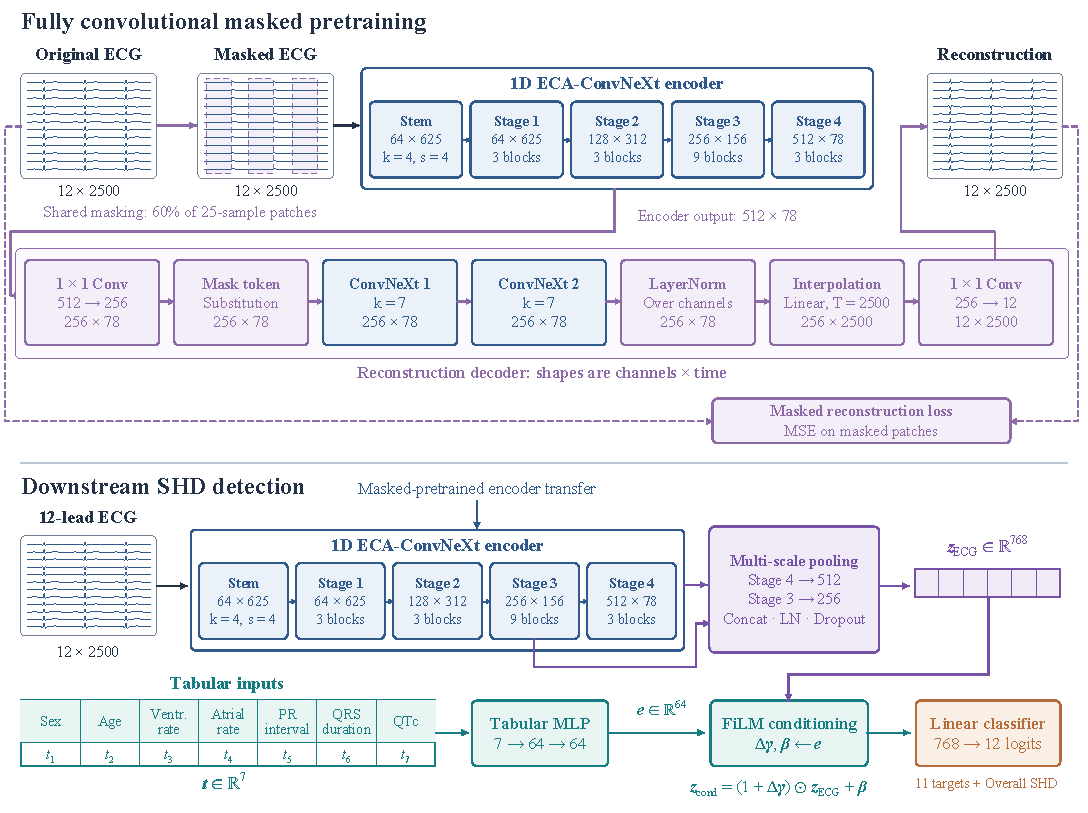
\includegraphics[width=\textwidth]{fig2_architecture_revised.pdf}
\caption{全卷积掩码预训练与下游一维 ECA--ConvNeXt 架构。同步十二导联波形采用跨导联共享的时间片段掩码，并仅在被遮蔽位置计算重建误差；下游阶段迁移掩码预训练编码器。stage 3 与 stage 4 特征经注意力汇聚后拼接为 768 维 ECG 表征，7 个表格变量通过 $\mathbf{z}_{\mathrm{cond}}=(\mathbf{1}+\Delta\boldsymbol{\gamma})\odot\mathbf{z}_{\mathrm{ECG}}+\boldsymbol{\beta}$ 进行 FiLM 条件调制，最终分类层输出一个 12 维 logit 向量。ECG 仅示意三个周期，实际模型输入仍为 $12\times2500$；形状省略批量维，表格单元格表示输入特征。}
\label{fig:architecture}
\end{bspcwidefigure}

\BSPCseparatearchitecturefigures

图~\ref{fig:module_details}展示 ECA--ConvNeXt 块、通道注意力、多尺度时间汇聚与Tabular inputs 条件调制。

\begin{bspcwidefigure}[!t]
\centering
\begin{minipage}[t]{0.49\textwidth}
  \centering
  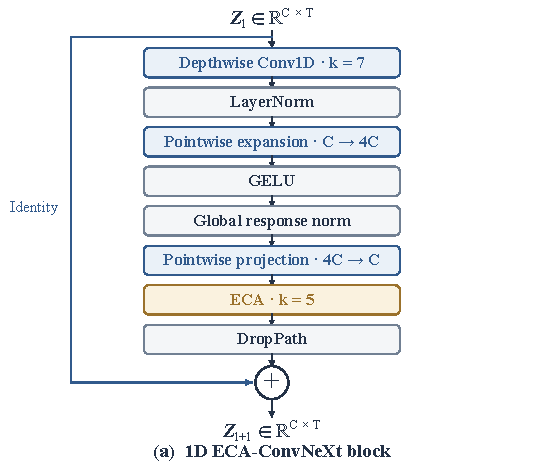
\includegraphics[width=\linewidth]{fig3a_eca_convnext_block_revised.pdf}
\end{minipage}\hfill
\begin{minipage}[t]{0.49\textwidth}
  \centering
  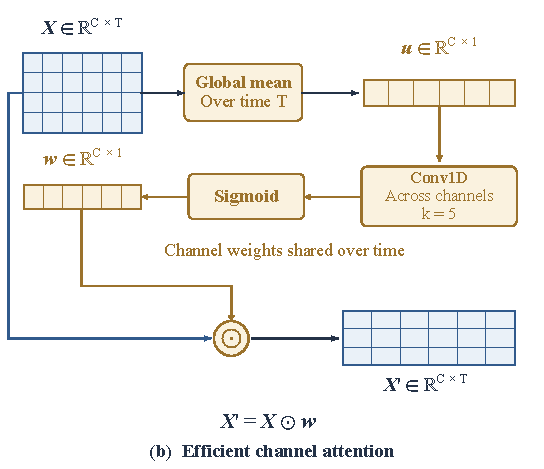
\includegraphics[width=\linewidth]{fig3b_eca_attention_module_revised.pdf}
\end{minipage}

\vspace{0.7em}

\begin{minipage}[t]{0.49\textwidth}
  \centering
  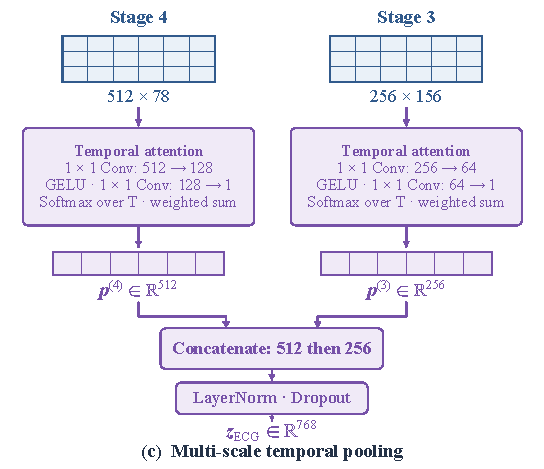
\includegraphics[width=\linewidth]{fig3c_multiscale_temporal_attention_revised.pdf}
\end{minipage}\hfill
\begin{minipage}[t]{0.49\textwidth}
  \centering
  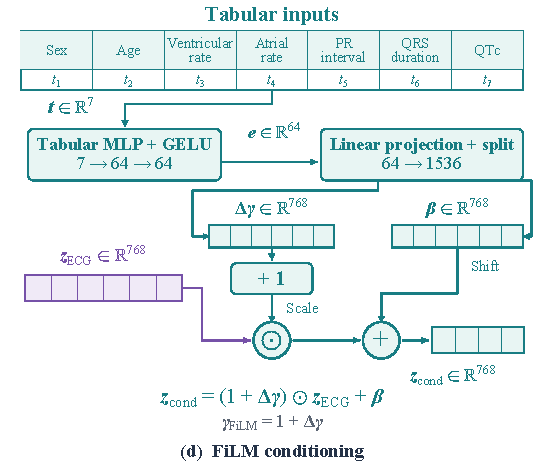
\includegraphics[width=\linewidth]{fig3d_film_conditioning_revised.pdf}
\end{minipage}
\caption{下游模型关键模块。子图 (a)--(d) 从左上至右下依次为：包含 GRN、ECA 和 DropPath 的一维 ECA--ConvNeXt 块；核大小 $k=5$ 的 ECA 通道注意力；仅汇聚 stage 3 与 stage 4 的多尺度时间注意力；以及由 7 个表格变量驱动的 FiLM 条件调制。}
\label{fig:module_details}
\end{bspcwidefigure}

\subsection{训练与模型选择}
\label{sec:training}

下游模型最多训练 100 个 epoch，批量大小为 64。优化器为 AdamW，$\beta^{\mathrm{Adam}}_1=0.9$、$\beta^{\mathrm{Adam}}_2=0.999$，初始学习率为 $10^{-3}$，权重衰减为 0.05，编码器按 0.75 的层级学习率衰减系数设置。学习率在前两个 epoch 线性预热，随后按余弦策略衰减；梯度范数裁剪阈值为 1.0，指数移动平均系数为 0.999。训练阶段对训练批次施加标准差为 0.05 的逐点高斯扰动，并随机选择 $10\%$ 离散时间索引在同一批次全部样本和导联上置零；验证集和测试集不使用增强。

模型选择以验证集 Overall SHD AUROC 为主要准则，连续 10 个 epoch 未改善时提前停止，并保存最佳指数移动平均权重。测试集仅在训练和模型选择结束后使用。下游实验使用随机种子 42、2026 和 3407，并采用确定性训练设置。

\subsection{实验比较}
\label{sec:comparisons}

主要比较为掩码预训练的 ECG-FCMAE 完整模型（Full）与同架构随机初始化对照（Strict）。两者使用相同的七个表格变量、数据划分、损失、优化、增强、训练预算和模型选择规则，实验变量为编码器初始化方式。标签效率实验使用 1\%、5\%、10\%、30\% 和 100\% 的有标签训练 ECG 记录；1\%--30\% 子集由同一固定记录排列的嵌套前缀构成，验证集和测试集保持不变。

输入与融合消融以 Full 为参照，设置仅 ECG（ECG-only，移除表格分支及 FiLM）、简单拼接（Concat，以拼接替代 FiLM）和仅表格变量（Tabular-only，移除 ECG 分支）三种配置，用于区分 ECG 信息、表格信息与融合方式对应的性能变化。严格匹配的架构组件消融分别移除 ECA（No ECA）、以全局平均汇聚替换时间注意力汇聚（GAP），或只保留 stage 4 表征（Stage-4 only）；十二导联输入、增强、数据划分和三个下游随机种子保持一致。另以 A--G 渐进链汇总初始化、ECA、汇聚尺度和表格变量融合的累积配置变化，其中 E、F、G 分别复用 ECG-only、Concat 和 Full 的结果。各预测目标的评价覆盖 11 种具体超声心动图异常和 Overall SHD。少导联分析采用真实通道切片与预训练 stem 权重选择，包括 6 个肢体导联、6 个胸前导联、I/II/V1/V5 四导联、单独 I 导联和单独 II 导联；各配置均重新进行下游训练，不进行少导联专用预训练。亚组分析按年龄、性别、种族/族裔和临床场景描述 Full 与 Strict 的测试集表现。

\subsection{统计分析}
\label{sec:statistics}

主要性能评价指标为测试集 Overall SHD 的受试者工作特征曲线下面积（AUROC），精确率--召回率曲线下面积（AUPRC）作为受测试集标签阳性率影响的补充性能评价指标。各预测目标的性能评价指标分别报告。排除 Overall SHD 后，11 种具体超声心动图异常 AUROC 的算术平均定义为 Macro-11 AUROC：
\begin{equation}
\mathrm{Macro\mbox{-}11\ AUROC}=\frac{1}{11}
\sum_{k=1}^{11}\mathrm{AUROC}_k.
\label{eq:macro11}
\end{equation}
Macro-11 与包含 Overall SHD 的 Macro-12 明确区分。

三个下游训练种子的均值与样本标准差描述训练变异。三种子集成取同一患者、同一目标的三个预测概率的算术平均。以测试患者为重采样单位，进行 2,000 次 percentile bootstrap，估计固定预测的 95\% 置信区间。模型比较使用相同重采样索引，差值定义为候选模型减参照模型；集成预测差值由原始预测的观测指标计算。患者级区间反映测试患者抽样不确定性，种子间标准差反映下游训练变异。亚组分析描述固定测试集中的模型表现。

\ifBSPCtwocolumn\else\FloatBarrier\fi

\section{结果}
\label{sec:results}

\subsection{测试队列与标签分布}
\label{sec:results_cohort}

测试集包含 $5{,}442$ 名患者，其中 $2{,}318$ 名患者的 Overall SHD 真实标签为阳性，测试集标签阳性率为 $42.5946\%$。11 种具体超声心动图异常的标签阳性率并不均一，因此分别评价 Overall SHD 和各预测目标的性能，并在解释低标签阳性率预测目标时同时考虑 AUROC、AUPRC、真实标签阳性数与区间宽度。

\subsection{预训练初始化消融}
\label{sec:results_primary}

三个下游训练种子中，Full 的 Overall SHD AUROC 为 $0.8521\pm0.0008$，Strict 为 $0.8448\pm0.0001$；对应 AUPRC 分别为 $0.8249\pm0.0009$ 和 $0.8149\pm0.0002$，Macro-11 AUROC 分别为 $0.8374\pm0.0020$ 和 $0.8258\pm0.0032$（表~\ref{tab:primary}）。

三种子概率集成后，Full 与 Strict 的 Overall SHD AUROC 分别为 0.8529 和 0.8468，观测差为 $+0.0061$，患者级配对 95\% 置信区间为 $[0.0034,\,0.0088]$。AUPRC 差值为 $+0.0082$（$[0.0042,\,0.0122]$），Macro-11 AUROC 差值为 $+0.0099$（$[0.0049,\,0.0153]$）。三个区间均高于 0，支持掩码预训练改善 SHD 判别性能。

\begin{table}[!htbp]
\centering
\BSPCtableformat

\caption{Full 与同架构随机初始化对照（Strict）的三种子结果。数值为三个下游训练种子的均值$\pm$样本标准差。}
\label{tab:primary}
\begin{tabularx}{\linewidth}{@{}Ycc@{}}
\toprule
性能评价指标 & Full & Strict \\
\midrule
SHD AUROC & 0.8521$\pm$0.0008 & 0.8448$\pm$0.0001 \\
SHD AUPRC & 0.8249$\pm$0.0009 & 0.8149$\pm$0.0002 \\
Macro-11 AUROC & 0.8374$\pm$0.0020 & 0.8258$\pm$0.0032 \\
\bottomrule
\end{tabularx}

\end{table}

\BSPCseparateresultfloatgroups

\subsection{标签效率}
\label{sec:results_label_efficiency}

预训练在五个有标签训练 ECG 记录比例下均提高了性能（表~\ref{tab:label_efficiency}；图~\ref{fig:label_efficiency}）。1\% 记录时，SSL 与 Scratch 的三种子 AUROC 分别为 $0.8003\pm0.0035$ 和 $0.7641\pm0.0130$；30\% 时分别为 $0.8447\pm0.0005$ 和 $0.8365\pm0.0027$；100\% 时分别为 $0.8521\pm0.0008$ 和 $0.8448\pm0.0001$。Scratch 在 1\% 条件下的种子间离散程度最大。

集成预测的 SSL$-$Scratch AUROC 差值在 1\%、5\%、10\%、30\% 和 100\% 条件下依次为 $+0.0323$、$+0.0196$、$+0.0127$、$+0.0055$ 和 $+0.0061$；相应配对 95\% 置信区间均排除 0（表~\ref{tab:label_paired}）。AUPRC 差值依次为 $+0.0579$、$+0.0339$、$+0.0204$、$+0.0112$ 和 $+0.0082$，其区间也均排除 0。AUROC 收益在 1\% 条件下最大，并随着有标签训练记录比例增加而总体减小，在 30\% 至 100\% 之间小幅回升；AUPRC 收益则随五个有标签训练记录比例依次减小。

\begin{table}[!htbp]
\centering
\BSPCtableformat

\caption{不同有标签训练 ECG 记录比例下的结果。数值为三个下游训练种子的均值$\pm$样本标准差；100\% 条件复用 Full/Strict。}
\label{tab:label_efficiency}
\begin{tabularx}{\linewidth}{@{}Ycc@{}}
\toprule
\multicolumn{3}{l}{\textit{(a) Overall SHD AUROC}} \\
比例 & SSL & Scratch \\
\midrule
1\% & 0.8003$\pm$0.0035 & 0.7641$\pm$0.0130 \\
5\% & 0.8250$\pm$0.0008 & 0.8001$\pm$0.0023 \\
10\% & 0.8350$\pm$0.0013 & 0.8181$\pm$0.0028 \\
30\% & 0.8447$\pm$0.0005 & 0.8365$\pm$0.0027 \\
100\% & 0.8521$\pm$0.0008 & 0.8448$\pm$0.0001 \\
\midrule
\multicolumn{3}{l}{\textit{(b) Overall SHD AUPRC}} \\
比例 & SSL & Scratch \\
\midrule
1\% & 0.7609$\pm$0.0054 & 0.6978$\pm$0.0215 \\
5\% & 0.7983$\pm$0.0012 & 0.7554$\pm$0.0054 \\
10\% & 0.8084$\pm$0.0013 & 0.7818$\pm$0.0037 \\
30\% & 0.8185$\pm$0.0006 & 0.8037$\pm$0.0029 \\
100\% & 0.8249$\pm$0.0009 & 0.8149$\pm$0.0002 \\
\bottomrule
\end{tabularx}

\end{table}

\begin{table}[!htbp]
\centering
\BSPCtableformat

\caption{标签效率的三种子概率集成比较。数值为观测 SSL$-$Scratch 差值及 2,000 次患者级配对 bootstrap 的 95\% CI；100\% 行采用标签效率分析的 bootstrap 区间。}
\label{tab:label_paired}
\begin{tabularx}{\linewidth}{@{}lZZ@{}}
\toprule
标注比例 & $\Delta$ SHD AUROC & $\Delta$ SHD AUPRC \\
\midrule
1\% & \shortstack{$0.0323$\\$[0.0239,\,0.0408]$} & \shortstack{$0.0579$\\$[0.0453,\,0.0707]$} \\
5\% & \shortstack{$0.0196$\\$[0.0134,\,0.0258]$} & \shortstack{$0.0339$\\$[0.0251,\,0.0425]$} \\
10\% & \shortstack{$0.0127$\\$[0.0077,\,0.0176]$} & \shortstack{$0.0204$\\$[0.0128,\,0.0282]$} \\
30\% & \shortstack{$0.0055$\\$[0.0017,\,0.0093]$} & \shortstack{$0.0112$\\$[0.0057,\,0.0167]$} \\
100\% & \shortstack{$0.0061$\\$[0.0034,\,0.0088]$} & \shortstack{$0.0082$\\$[0.0044,\,0.0122]$} \\
\bottomrule
\end{tabularx}

\end{table}
\begin{bspclabelefficiencyfigure}
\centering
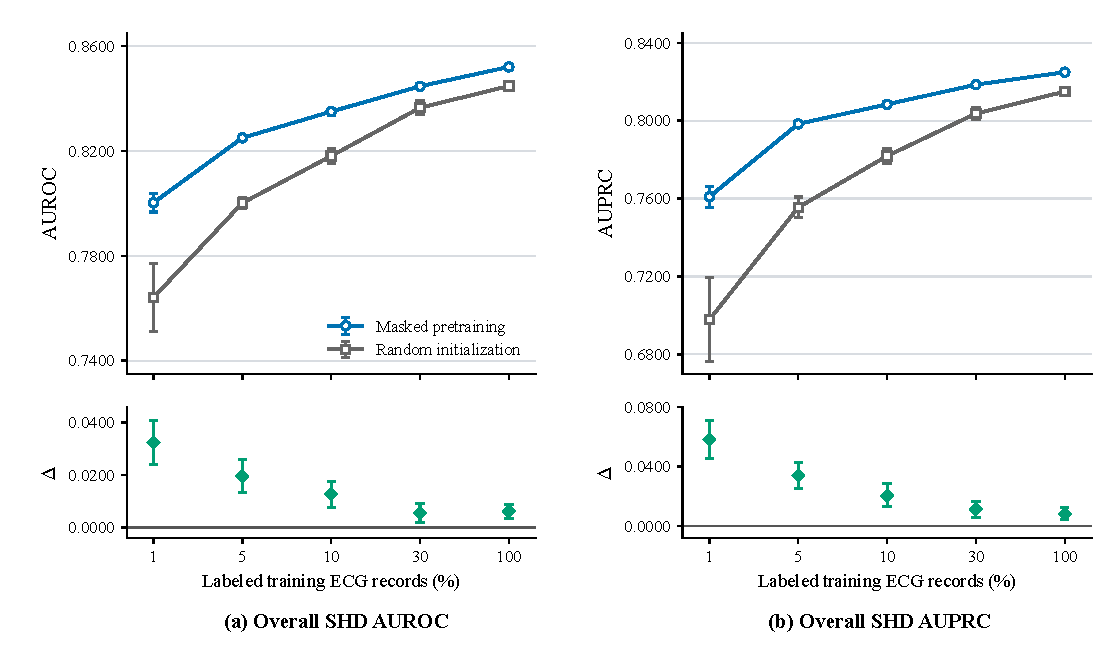
\includegraphics[width=0.8800\textwidth]{fig4_label_efficiency_revised.pdf}
\caption{不同有标签训练 ECG 记录比例下的 Overall SHD 表现。左、右两部分分别展示 AUROC 和 AUPRC；模型曲线为三个下游种子的均值，误差线为样本标准差。各面板下方的差值视图基于三种子概率集成，显示 SSL$-$Scratch 的观测差及 2,000 次患者级配对 bootstrap 的 95\% 置信区间。}
\label{fig:label_efficiency}
\end{bspclabelefficiencyfigure}

\BSPCseparateresultfloatgroups

\subsection{输入与融合消融实验}
\label{sec:results_structured}

输入与融合消融显示，ECG 波形是主要判别信息来源，而 7 个表格变量在完整模型中提供了补充信息（表~\ref{tab:modalities}）。Full、ECG-only 和 Tabular-only 的三种子 Overall SHD AUROC 分别为 $0.8521\pm0.0008$、$0.8466\pm0.0006$ 和 $0.7587\pm0.0006$。

Concat 的三种子 AUROC 为 $0.8505\pm0.0008$，接近 Full。

\begin{table}[!htbp]
\centering
\BSPCtableformat

\caption{输入与融合消融的三种子测试结果。Full 使用 ECG、7 个表格变量和 FiLM；ECG-only 移除表格分支及 FiLM，Concat 以简单拼接替代 FiLM，Tabular-only 移除 ECG 分支。}
\label{tab:modalities}
\begin{tabularx}{\linewidth}{@{}Yccc@{}}
\toprule
模型 & SHD AUROC & SHD AUPRC & \shortstack{Macro-11\\AUROC} \\
\midrule
Full & 0.8521$\pm$0.0008 & 0.8249$\pm$0.0009 & 0.8374$\pm$0.0020 \\
ECG-only & 0.8466$\pm$0.0006 & 0.8214$\pm$0.0006 & 0.8297$\pm$0.0025 \\
Concat & 0.8505$\pm$0.0008 & 0.8224$\pm$0.0009 & 0.8348$\pm$0.0002 \\
Tabular-only & 0.7587$\pm$0.0006 & 0.7002$\pm$0.0018 & 0.7281$\pm$0.0018 \\
\bottomrule
\end{tabularx}

\end{table}

\subsection{架构组件消融实验}
\label{sec:results_architecture_ablation}

组件消融的点估计接近 Full（表~\ref{tab:architecture_ablation}）。No ECA、GAP 和 Stage-4 only 的 Overall SHD AUROC 分别为 $0.8519\pm0.0003$、$0.8517\pm0.0004$ 和 $0.8517\pm0.0005$，Full 为 $0.8521\pm0.0008$。

A--G 累积组件链的 AUROC 从 A 的 $0.8390\pm0.0021$（随机初始化、无 ECA、stage-4 GAP、无表格变量融合）变化至 G 的 $0.8521\pm0.0008$（Full）。表~\ref{tab:component_chain} 汇总累积配置及其平均性能。

\begin{table}[!htbp]
\centering
\BSPCtableformat

\caption{严格匹配的架构组件消融。数值为三种子均值$\pm$样本标准差。Strict 仅改变预训练初始化；No ECA 移除 ECA；GAP 以全局平均汇聚替代时间注意力汇聚；Stage-4 only 移除 stage-3 聚合路径。}
\label{tab:architecture_ablation}
\begin{tabularx}{\linewidth}{@{}Yccc@{}}
\toprule
配置 & SHD AUROC & SHD AUPRC & \shortstack{Macro-11\\AUROC} \\
\midrule
Full & 0.8521$\pm$0.0008 & 0.8249$\pm$0.0009 & 0.8374$\pm$0.0020 \\
\BSPCstrictnopretraining & 0.8448$\pm$0.0001 & 0.8149$\pm$0.0002 & 0.8258$\pm$0.0032 \\
No ECA & 0.8519$\pm$0.0003 & 0.8262$\pm$0.0014 & 0.8366$\pm$0.0003 \\
GAP & 0.8517$\pm$0.0004 & 0.8240$\pm$0.0012 & 0.8366$\pm$0.0019 \\
Stage-4 only & 0.8517$\pm$0.0005 & 0.8253$\pm$0.0017 & 0.8379$\pm$0.0007 \\
\bottomrule
\end{tabularx}

\end{table}

\begin{bspcwidetable}[!htbp]
\centering
\BSPCtableformat

\caption{A--G 渐进组件链。每行同时列出累积配置及其三种子均值$\pm$样本标准差。E、F、G 分别复用 ECG-only、Concat 和 Full。}
\label{tab:component_chain}
\begin{tabularx}{\textwidth}{@{}cYcYcccc@{}}
\toprule
组 & 初始化 & ECA & 汇聚 / 尺度 & 表格融合 & \shortstack{SHD\\AUROC} & \shortstack{SHD\\AUPRC} & \shortstack{Macro-11\\AUROC} \\
\midrule
A & Scratch & Off & Stage-4 GAP & None & 0.8390$\pm$0.0021 & 0.8106$\pm$0.0029 & 0.8236$\pm$0.0032 \\
B & FCMAE no-ECA & Off & Stage-4 GAP & None & 0.8459$\pm$0.0008 & 0.8221$\pm$0.0006 & 0.8290$\pm$0.0011 \\
C & FCMAE\allowbreak(ECA) & On & Stage-4 GAP & None & 0.8466$\pm$0.0003 & 0.8211$\pm$0.0011 & 0.8299$\pm$0.0006 \\
D & FCMAE\allowbreak(ECA) & On & Stage-4 attention & None & 0.8470$\pm$0.0006 & 0.8218$\pm$0.0009 & 0.8307$\pm$0.0005 \\
E & FCMAE\allowbreak(ECA) & On & Stage-3/4 attention & None & 0.8466$\pm$0.0006 & 0.8214$\pm$0.0006 & 0.8297$\pm$0.0025 \\
F & FCMAE\allowbreak(ECA) & On & Stage-3/4 attention & Concat & 0.8505$\pm$0.0008 & 0.8224$\pm$0.0009 & 0.8348$\pm$0.0002 \\
G & FCMAE\allowbreak(ECA) & On & Stage-3/4 attention & FiLM & 0.8521$\pm$0.0008 & 0.8249$\pm$0.0009 & 0.8374$\pm$0.0020 \\
\bottomrule
\end{tabularx}

\end{bspcwidetable}

\BSPCseparateresultfloatgroups

\subsection{与已报道 EchoNext 模型的比较}
\label{sec:results_published_comparison}

已报道的 EchoNext 研究分别报告了 Overall SHD 预测目标和 11 种具体异常的 Macro-11 AUROC。EchoNext-Mini 使用十二导联 ECG 与 7 个表格变量，可解释广义加性模型使用 71 个 ECG 基础模型预测量与相同的 7 个表格变量；两项研究报告的 Overall SHD AUROC 分别为 0.8200 和 0.8280\cite{hughes2026echonextmini,zhou2026gamshd}。统一 EchoNext 基准在相同标签体系下比较了多种微调基础模型和监督模型，其 ECG-only Macro-11 AUROC 为 $[0.7720,\,0.8310]$\cite{almasud2026benchmark}。表~\ref{tab:published_comparison} 将这些公开数值与本研究的三种子结果并列展示。

\begin{table}[!htbp]
\centering
\BSPCtableformat

\caption{已报道 EchoNext 结果与 ECG-FCMAE。文献结果采用各原研究协议；本文结果为三种子均值$\pm$样本标准差。T 表示七个表格变量，P 表示 71 个 ECG 基础模型预测量。}
\label{tab:published_comparison}
\begin{tabularx}{\linewidth}{@{}Yp{0.1900\linewidth}r@{}}
\toprule
Method & Input & AUROC \\
\midrule
\multicolumn{3}{@{}l}{\textit{(a) Overall SHD AUROC}} \\
EchoNext-Mini\cite{hughes2026echonextmini} & ECG + T & 0.8200 \\
Interpretable GAM\cite{zhou2026gamshd} & P + T & 0.8280 \\
\midrule
\textbf{ECG-FCMAE (Ours)} & ECG + T & 0.8521$\pm$0.0008 \\
\midrule
\multicolumn{3}{@{}l}{\textit{(b) Macro-11 AUROC}} \\
\multicolumn{3}{@{}l}{Fine-tuned foundation models\cite{almasud2026benchmark}} \\
ECGFounder & ECG & 0.8170 \\
ECG-JEPA & ECG & 0.8170 \\
ST-MEM & ECG & 0.8160 \\
MERL & ECG & 0.8220 \\
ECGFM-KED & ECG & 0.8060 \\
HuBERT-ECG & ECG & 0.7920 \\
ECG-FM & ECG & 0.7720 \\
ECG-CPC & ECG & 0.8310 \\
\addlinespace
\multicolumn{3}{@{}l}{Supervised models\cite{almasud2026benchmark}} \\
S4 & ECG & 0.8190 \\
Net1D & ECG & 0.8030 \\
\midrule
\textbf{ECG-FCMAE, ECG-only (Ours)} & ECG & 0.8297$\pm$0.0025 \\
\textbf{ECG-FCMAE (Ours)} & ECG + T & 0.8374$\pm$0.0020 \\
\bottomrule
\end{tabularx}

\end{table}

ECG-FCMAE 的三种子 Overall SHD AUROC 为 $0.8521\pm0.0008$。ECG-only 变体的 Macro-11 AUROC 为 $0.8297\pm0.0025$，接近统一基准中 ECG-CPC 的 0.8310；加入七个表格变量后，完整模型达到 $0.8374\pm0.0020$。

\BSPCseparateresultfloatgroups

\subsection{各预测目标的性能}
\label{sec:results_endpoints}

完整模型的三随机种子概率集成在不同预测目标上的判别性能存在明显异质性（图~\ref{fig:endpoint_performance}；表~\ref{tab:endpoints}）。11 种具体超声心动图异常的 AUROC 从中度及以上主动脉瓣反流的 0.7717 到 LVEF $\leq45\%$ 的 0.9081；AUPRC 从中度及以上主动脉瓣反流的 0.0514 到 LVEF $\leq45\%$ 的 0.7470。中度及以上右心室收缩功能障碍和中度及以上主动脉瓣狭窄的 AUROC 分别为 0.8995 和 0.8895，而中度及以上肺动脉瓣反流、中度及以上主动脉瓣反流以及中量或大量心包积液的 AUPRC 较低且区间较宽。这些目标的低标签阳性率对应较低的 AUPRC 和较宽的估计区间。

\begin{bspcwidefigure}[t]
\centering
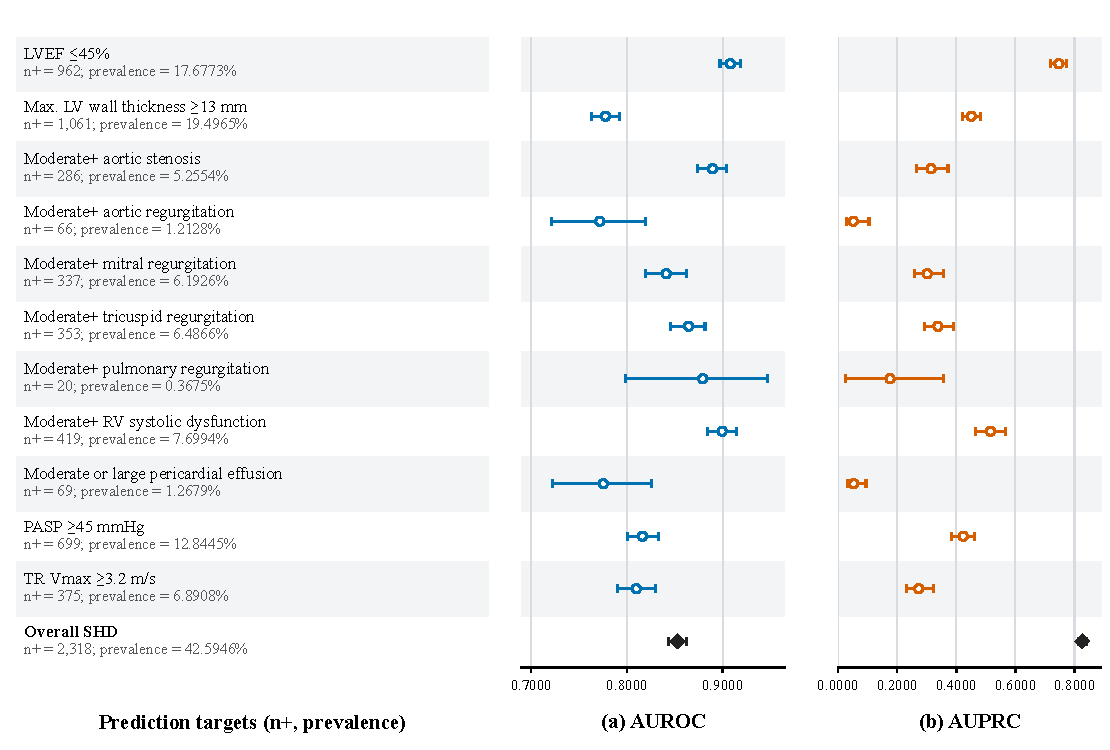
\includegraphics[width=0.9600\textwidth]{fig5_endpoint_performance_revised.pdf}
\caption{完整模型的三随机种子概率集成在 11 种具体超声心动图异常和 Overall SHD 上的判别性能。点和横线分别表示 AUROC 或 AUPRC 的点估计及 2,000 次患者级 bootstrap 95\% 置信区间；图中同时给出各预测目标的真实标签阳性数与测试集标签阳性率，以辅助解释低标签阳性率预测目标的区间宽度和较低 AUPRC。}
\label{fig:endpoint_performance}
\end{bspcwidefigure}

\begin{bspcwidetable}[!tbp]
\centering
\BSPCtableformat

\caption{完整模型的三随机种子概率集成在各预测目标上的结果。区间为 2,000 次患者级 bootstrap 的 95\% 置信区间。}
\label{tab:endpoints}
\begin{tabularx}{\textwidth}{Ycc}
\toprule
预测目标 & AUROC（95\% CI） & AUPRC（95\% CI） \\
\midrule
LVEF $\leq45\%$ & 0.9081 $[0.8973,\,0.9189]$ & 0.7470 $[0.7194,\,0.7728]$ \\
左心室壁厚增加（室间隔或左心室后壁舒张期厚度的较大值 $\geq13$~mm） & 0.7775 $[0.7628,\,0.7921]$ & 0.4508 $[0.4207,\,0.4821]$ \\
中度及以上主动脉瓣狭窄 & 0.8895 $[0.8734,\,0.9044]$ & 0.3146 $[0.2665,\,0.3719]$ \\
中度及以上主动脉瓣反流 & 0.7717 $[0.7208,\,0.8196]$ & 0.0514 $[0.0301,\,0.1047]$ \\
中度及以上二尖瓣反流 & 0.8410 $[0.8190,\,0.8621]$ & 0.3015 $[0.2580,\,0.3554]$ \\
中度及以上三尖瓣反流 & 0.8645 $[0.8458,\,0.8816]$ & 0.3378 $[0.2930,\,0.3906]$ \\
中度及以上肺动脉瓣反流 & 0.8793 $[0.7988,\,0.9474]$ & 0.1759 $[0.0243,\,0.3579]$ \\
中度及以上右心室收缩功能障碍 & 0.8995 $[0.8838,\,0.9145]$ & 0.5157 $[0.4656,\,0.5664]$ \\
中量或大量心包积液 & 0.7752 $[0.7221,\,0.8258]$ & 0.0530 $[0.0337,\,0.0945]$ \\
PASP $\geq45$ mmHg & 0.8162 $[0.8004,\,0.8326]$ & 0.4233 $[0.3839,\,0.4608]$ \\
TR Vmax $\geq3.2$ m/s & 0.8098 $[0.7900,\,0.8298]$ & 0.2728 $[0.2311,\,0.3216]$ \\
Overall SHD & 0.8529 $[0.8431,\,0.8627]$ & 0.8263 $[0.8120,\,0.8403]$ \\
\bottomrule
\end{tabularx}

\end{bspcwidetable}

\BSPCkeependpointorder

\subsection{少导联分析}
\label{sec:results_reduced_leads}

所有少导联模型均在真实通道切片后重新进行下游训练。Limb-6、Precordial-6、Anatomical-4、Lead-I 和 Lead-II 的三种子 Overall SHD AUROC 分别为 $0.8322\pm0.0016$、$0.8463\pm0.0003$、$0.8465\pm0.0006$、$0.8245\pm0.0005$ 和 $0.8196\pm0.0005$；对应 AUPRC 分别为 $0.8007\pm0.0024$、$0.8192\pm0.0005$、$0.8208\pm0.0013$、$0.7962\pm0.0002$ 和 $0.7783\pm0.0005$。Precordial-6 与 Anatomical-4 在五种配置中最接近十二导联 Full。

表~\ref{tab:reduced_summary} 汇总五种少导联配置的性能。各配置较低的平均 AUROC 量化了减少输入通道后的性能下降。

\begin{table}[!htbp]
\centering
\BSPCtableformat

\caption{少导联测试性能，数值为三种子均值$\pm$样本标准差。Limb-6 使用 I、II、III、aVR、aVL、aVF；Precordial-6 使用 V1--V6；Anatomical-4 使用 I、II、V1、V5。}
\label{tab:reduced_summary}
\begin{tabularx}{\linewidth}{@{}Yccc@{}}
\toprule
配置 & SHD AUROC & SHD AUPRC & \shortstack{Macro-11\\AUROC} \\
\midrule
Limb-6 & 0.8322$\pm$0.0016 & 0.8007$\pm$0.0024 & 0.8087$\pm$0.0043 \\
Precordial-6 & 0.8463$\pm$0.0003 & 0.8192$\pm$0.0005 & 0.8306$\pm$0.0011 \\
Anatomical-4 & 0.8465$\pm$0.0006 & 0.8208$\pm$0.0013 & 0.8314$\pm$0.0012 \\
Lead-I & 0.8245$\pm$0.0005 & 0.7962$\pm$0.0002 & 0.7942$\pm$0.0052 \\
Lead-II & 0.8196$\pm$0.0005 & 0.7783$\pm$0.0005 & 0.7857$\pm$0.0024 \\
\bottomrule
\end{tabularx}

\end{table}

\subsection{支持性亚组分析}
\label{sec:results_subgroups}

在 16 个预定义的年龄、性别、种族/族裔及临床场景亚组中，Full 相对 Strict 的 AUROC 点差在 15 个亚组为正，9 个患者级配对 95\% 置信区间排除 0。70--79 岁组的差值最大，为 $+0.0134$（$[0.0066,\,0.0204]$）；Asian 亚组为 $-0.0022$（$[-0.0210,\,0.0152]$）。Asian 与 Procedural 等较小亚组的区间较宽。完整结果见表~\ref{tab:subgroups}。

\begin{bspcwidetable}[!htbp]
\centering
\BSPCtableformat

\caption{预定义亚组的三种子概率集成结果。各单元格为估计值及 2,000 次患者级 bootstrap 的 95\% CI；$\Delta$ AUROC 为 Full$-$Strict。计数为患者数 / SHD 阳性患者数，阳性率为两者之比。AUPRC 与对应亚组阳性率同时报告。}
\label{tab:subgroups}
\begin{tabularx}{\textwidth}{@{}Ycccccc@{}}
\toprule
亚组 & $n/n_+$ & 阳性率 & \shortstack{Strict\\AUROC} & \shortstack{Full\\AUROC} & \shortstack{Full\\AUPRC} & $\Delta$ AUROC \\
\midrule
\multicolumn{7}{@{}l}{\textit{年龄}} \\
18--59 & 2124/671 & 0.3159 & \shortstack{$0.8560$\\$[0.8390,\,0.8730]$} & \shortstack{$0.8610$\\$[0.8440,\,0.8780]$} & \shortstack{$0.7780$\\$[0.7460,\,0.8060]$} & \shortstack{$0.0048$\\$[-0.0003,\,0.0096]$} \\
60--69 & 1318/524 & 0.3976 & \shortstack{$0.8390$\\$[0.8170,\,0.8600]$} & \shortstack{$0.8480$\\$[0.8260,\,0.8680]$} & \shortstack{$0.8080$\\$[0.7760,\,0.8380]$} & \shortstack{$0.0086$\\$[0.0025,\,0.0145]$} \\
70--79 & 1154/578 & 0.5009 & \shortstack{$0.8010$\\$[0.7760,\,0.8250]$} & \shortstack{$0.8150$\\$[0.7890,\,0.8380]$} & \shortstack{$0.8380$\\$[0.8100,\,0.8630]$} & \shortstack{$0.0134$\\$[0.0066,\,0.0204]$} \\
80+ & 846/545 & 0.6442 & \shortstack{$0.7860$\\$[0.7540,\,0.8160]$} & \shortstack{$0.7890$\\$[0.7570,\,0.8180]$} & \shortstack{$0.8780$\\$[0.8530,\,0.9010]$} & \shortstack{$0.0029$\\$[-0.0064,\,0.0125]$} \\
\midrule
\multicolumn{7}{@{}l}{\textit{性别}} \\
Female & 2731/1001 & 0.3665 & \shortstack{$0.8470$\\$[0.8320,\,0.8620]$} & \shortstack{$0.8520$\\$[0.8370,\,0.8660]$} & \shortstack{$0.7890$\\$[0.7640,\,0.8120]$} & \shortstack{$0.0049$\\$[0.0007,\,0.0090]$} \\
Male & 2711/1317 & 0.4858 & \shortstack{$0.8410$\\$[0.8260,\,0.8550]$} & \shortstack{$0.8480$\\$[0.8340,\,0.8630]$} & \shortstack{$0.8520$\\$[0.8330,\,0.8690]$} & \shortstack{$0.0077$\\$[0.0038,\,0.0116]$} \\
\midrule
\multicolumn{7}{@{}l}{\textit{种族/族裔}} \\
Hispanic & 1649/620 & 0.3760 & \shortstack{$0.8470$\\$[0.8280,\,0.8660]$} & \shortstack{$0.8540$\\$[0.8350,\,0.8710]$} & \shortstack{$0.8050$\\$[0.7770,\,0.8320]$} & \shortstack{$0.0064$\\$[0.0015,\,0.0117]$} \\
White & 1569/656 & 0.4181 & \shortstack{$0.8370$\\$[0.8180,\,0.8580]$} & \shortstack{$0.8430$\\$[0.8240,\,0.8630]$} & \shortstack{$0.8110$\\$[0.7830,\,0.8380]$} & \shortstack{$0.0061$\\$[0.0005,\,0.0115]$} \\
Black & 846/405 & 0.4787 & \shortstack{$0.8470$\\$[0.8200,\,0.8710]$} & \shortstack{$0.8520$\\$[0.8250,\,0.8770]$} & \shortstack{$0.8550$\\$[0.8250,\,0.8840]$} & \shortstack{$0.0055$\\$[-0.0011,\,0.0123]$} \\
Asian & 153/70 & 0.4575 & \shortstack{$0.8480$\\$[0.7840,\,0.9070]$} & \shortstack{$0.8460$\\$[0.7820,\,0.9050]$} & \shortstack{$0.8240$\\$[0.7310,\,0.9010]$} & \shortstack{$-0.0022$\\$[-0.0210,\,0.0152]$} \\
Other & 457/200 & 0.4376 & \shortstack{$0.8480$\\$[0.8130,\,0.8820]$} & \shortstack{$0.8530$\\$[0.8200,\,0.8860]$} & \shortstack{$0.8300$\\$[0.7810,\,0.8780]$} & \shortstack{$0.0055$\\$[-0.0043,\,0.0161]$} \\
Unknown & 768/367 & 0.4779 & \shortstack{$0.8540$\\$[0.8270,\,0.8800]$} & \shortstack{$0.8630$\\$[0.8360,\,0.8870]$} & \shortstack{$0.8530$\\$[0.8160,\,0.8870]$} & \shortstack{$0.0085$\\$[0.0011,\,0.0158]$} \\
\midrule
\multicolumn{7}{@{}l}{\textit{临床场景}} \\
Emergency & 1971/788 & 0.3998 & \shortstack{$0.8510$\\$[0.8350,\,0.8680]$} & \shortstack{$0.8580$\\$[0.8420,\,0.8740]$} & \shortstack{$0.8120$\\$[0.7850,\,0.8380]$} & \shortstack{$0.0064$\\$[0.0018,\,0.0108]$} \\
Inpatient & 2203/1156 & 0.5247 & \shortstack{$0.8220$\\$[0.8040,\,0.8400]$} & \shortstack{$0.8290$\\$[0.8120,\,0.8450]$} & \shortstack{$0.8560$\\$[0.8370,\,0.8730]$} & \shortstack{$0.0066$\\$[0.0014,\,0.0118]$} \\
Outpatient & 1059/271 & 0.2559 & \shortstack{$0.8300$\\$[0.8000,\,0.8580]$} & \shortstack{$0.8370$\\$[0.8060,\,0.8650]$} & \shortstack{$0.7140$\\$[0.6620,\,0.7640]$} & \shortstack{$0.0068$\\$[-0.0003,\,0.0137]$} \\
Procedural & 209/103 & 0.4928 & \shortstack{$0.8380$\\$[0.7850,\,0.8880]$} & \shortstack{$0.8500$\\$[0.7950,\,0.8970]$} & \shortstack{$0.8370$\\$[0.7640,\,0.9000]$} & \shortstack{$0.0115$\\$[-0.0047,\,0.0284]$} \\
\bottomrule
\end{tabularx}

\end{bspcwidetable}

\section{讨论}
\label{sec:discussion}

\subsection{主要发现}
\label{sec:discussion_findings}

掩码预训练提高了 EchoNext 中 Overall SHD AUROC、AUPRC 和 Macro-11 AUROC。Full 的三种子均值和概率集成结果均高于 Strict，集成预测的患者级配对区间排除 0。预训练优势覆盖 1\%--100\% 的有标签训练记录，且在 1\% 时最大。输入消融表明 ECG 提供主要判别信息，表格变量提供补充信息；各预测目标及导联配置表现出不同的性能水平。

\subsection{掩码预训练与 ECG 表征学习}
\label{sec:discussion_representation}

共享时间片段掩码要求编码器结合未遮蔽的时间上下文与同步导联信息，重建缺失片段。既往心电图掩码模型也利用时间或导联维度的上下文开展下游迁移\cite{zhang2023maefe,na2024stmem,ran_joint_masking_2024,sawano_masked_lvsd_2024}。匹配比较与标签效率结果支持重建任务在接触下游标签前学习可复用的 ECG 表征。

三种子标准差描述共享同一预训练检查点时的下游训练变异，患者级 bootstrap 则描述固定集成预测的测试患者抽样不确定性。两类估计从训练重复与患者抽样两个层面刻画预训练优势。

移除 ECA、以 GAP 替代注意力汇聚或只保留 stage 4 后，点估计与 Full 接近。A--G 组件链以 Full 为参照，补充展示累积设计变化对应的性能趋势。

\subsection{与既往 ECG 表征学习研究的关系}
\label{sec:discussion_prior}

既往监督式人工智能心电图研究已评价单一结构异常、瓣膜病和范围更广的 SHD\cite{attia2019contractile,elias2022valvenet,ulloacerna2022rechommend,poterucha2025echonext,dhingra_present_shd_2025}，自监督研究则通过对比学习、导联关系建模、变换判别和掩码重建学习标签无关的 ECG 表示\cite{kiyasseh2021clocs,mehari2022ssl,oh2022leadagnostic,zhang_reverse_2023,zhang2023maefe,na2024stmem}。本研究连接了这两条证据线：在超声心动图定义的多目标二分类任务中，直接检验掩码卷积预训练相对同架构随机初始化的增量价值，并显式评价标签效率。

预训练优势覆盖五个标注比例，SSL 与 Scratch 的配对 AUROC 和 AUPRC 区间均排除 0。AUROC 差值在 1\% 时最大，随后总体下降，在 30\% 至 100\% 之间略有回升；AUPRC 差值随标注比例增加持续下降。

\subsection{表格信息与少导联结果}
\label{sec:discussion_secondary}

ECG-only 高于 Tabular-only，Full 高于 ECG-only，表明 ECG 波形提供主要判别信息，七个表格变量提供补充信息。多模态 ECG 研究也将融合效果与输入表示和预测目标相联系\cite{jiang_multimodal_lqts_2024,narotamo_multimodal_2024}。FiLM 与简单拼接的平均性能接近。

减少输入通道降低了 Overall SHD AUROC。Precordial-6 和 Anatomical-4 在五种少导联配置中保留的性能最多。这些重新训练的配置刻画了 SHD 判别对通道可用性的敏感性，并补充了既往少导联分类和单导联 SHD 检测研究\cite{le_lightx3ecg_2023,aminorroaya_adapt_shd_2025}。

\subsection{临床相关性}
\label{sec:discussion_clinical}

ECG 来源的 SHD 概率为超声心动图检查的优先排序提供了依据，超声心动图用于确认结构异常。外部校准、决策分析和前瞻性流程评价可量化这一排序策略的临床价值。

\subsection{局限性}
\label{sec:limitations}

本研究使用单中心回顾性配对队列。标签效率子集按 ECG 记录抽样，训练集允许同一患者贡献多条记录。三个下游种子共享一个预训练检查点，其离散程度估计下游训练变异。不同预测目标的标签阳性率和区间宽度差异较大，较小亚组的区间也更宽。

数据发布提供处理后的数组，但缺少完整的队列构建与重复超声检查选择流程、原始波形转数组代码、滤波参数、预处理拟合人群和统计量，以及表格变量缩放和缺失值处理实现。这些上游细节的缺失限制了完整数据流程的重建。独立预训练重复和外部队列可评价预训练变异与迁移性，前瞻性研究可评价校准和决策效用。

\FloatBarrier
\section{结论}
\label{sec:conclusion}

ECG-FCMAE 提高了 EchoNext 中十二导联 ECG 对超声心动图定义 SHD 的检测性能。相对随机初始化，三种子概率集成的 Overall SHD AUROC 增加 $0.0061$（患者级配对 95\% 置信区间：$[0.0034,\,0.0088]$）。预训练在 1\%--100\% 的有标签训练记录范围内均提高性能，最大收益出现在 1\%。输入消融显示 ECG 波形提供主要判别信息，表格变量带来补充价值。终点分析与少导联分析进一步刻画了性能随预测任务和可用通道的变化。



\BSPCprintbibliography

\end{document}
